OpenID Connect (OIDC) is a simple identity layer~\cite{siriwardenaOpenid2020, sakimuraOpenid2014}
on top of the OAuth 2.0 protocol~\cite{hardt2012oauth}.
It enables Clients to verify the identity of the End-User based on the authentication performed by an Authorization Server,
as well as to obtain basic profile information about the End-User in an interoperable and REST-like manner.

OAuth 2.0 is a protocol that enables a third-party application to obtain limited access to an HTTP service,
either on behalf of a resource owner by orchestrating an approval interaction between the resource owner
and the HTTP service, or by allowing the third-party application to obtain access on its own behalf.

OAuth 2.0 provides various standardized message flows based on JSON and HTTP;
OpenID Connect uses them to provide identity services.

The problem OAuth 2.0 solves is that in the traditional client-server authentication model,
the client requests an access-restricted resource
on the server by authenticating with the server using the resource owner's credentials.
In order to provide third-party applications access to restricted resources,
the resource owner shares its credentials with the third party.
This creates several problems and limitations~\cite{hardt2012oauth}:
\begin{itemize}
    \item Third-party applications are required to store the resource owner's credentials for future use, typically
    a password in clear-text.
    \item Servers are required to support password authentication, despite the security weaknesses inherent in passwords.
    \item Third-party applications gain overly broad access to the resource owner's protected resources,
    leaving resource owners without any ability to restrict duration or access to a limited subset of resources.
    \item Resource owners cannot revoke access to an individual third party without revoking access to all third parties,
    and must do so by changing the third party's password.
    \item Compromise of any third-party application results in compromise of the end-user's password
    and all the data protected by that password.
\end{itemize}
OAuth 2.0 addresses these issues by introducing an authorization layer and separating the role of the client
from that of the resource owner.
In OAuth, the client requests access to resources controlled by the resource owner and hosted by the resource server.
Instead of using the resource owner's credentials to access protected resources, the client obtains an access token.
OAuth 2.0 with the Proof of Key Code Exchange~\cite{bradley2015rfc} flow is displayed on the diagram below
\begin{figure}[H]
    \centering
    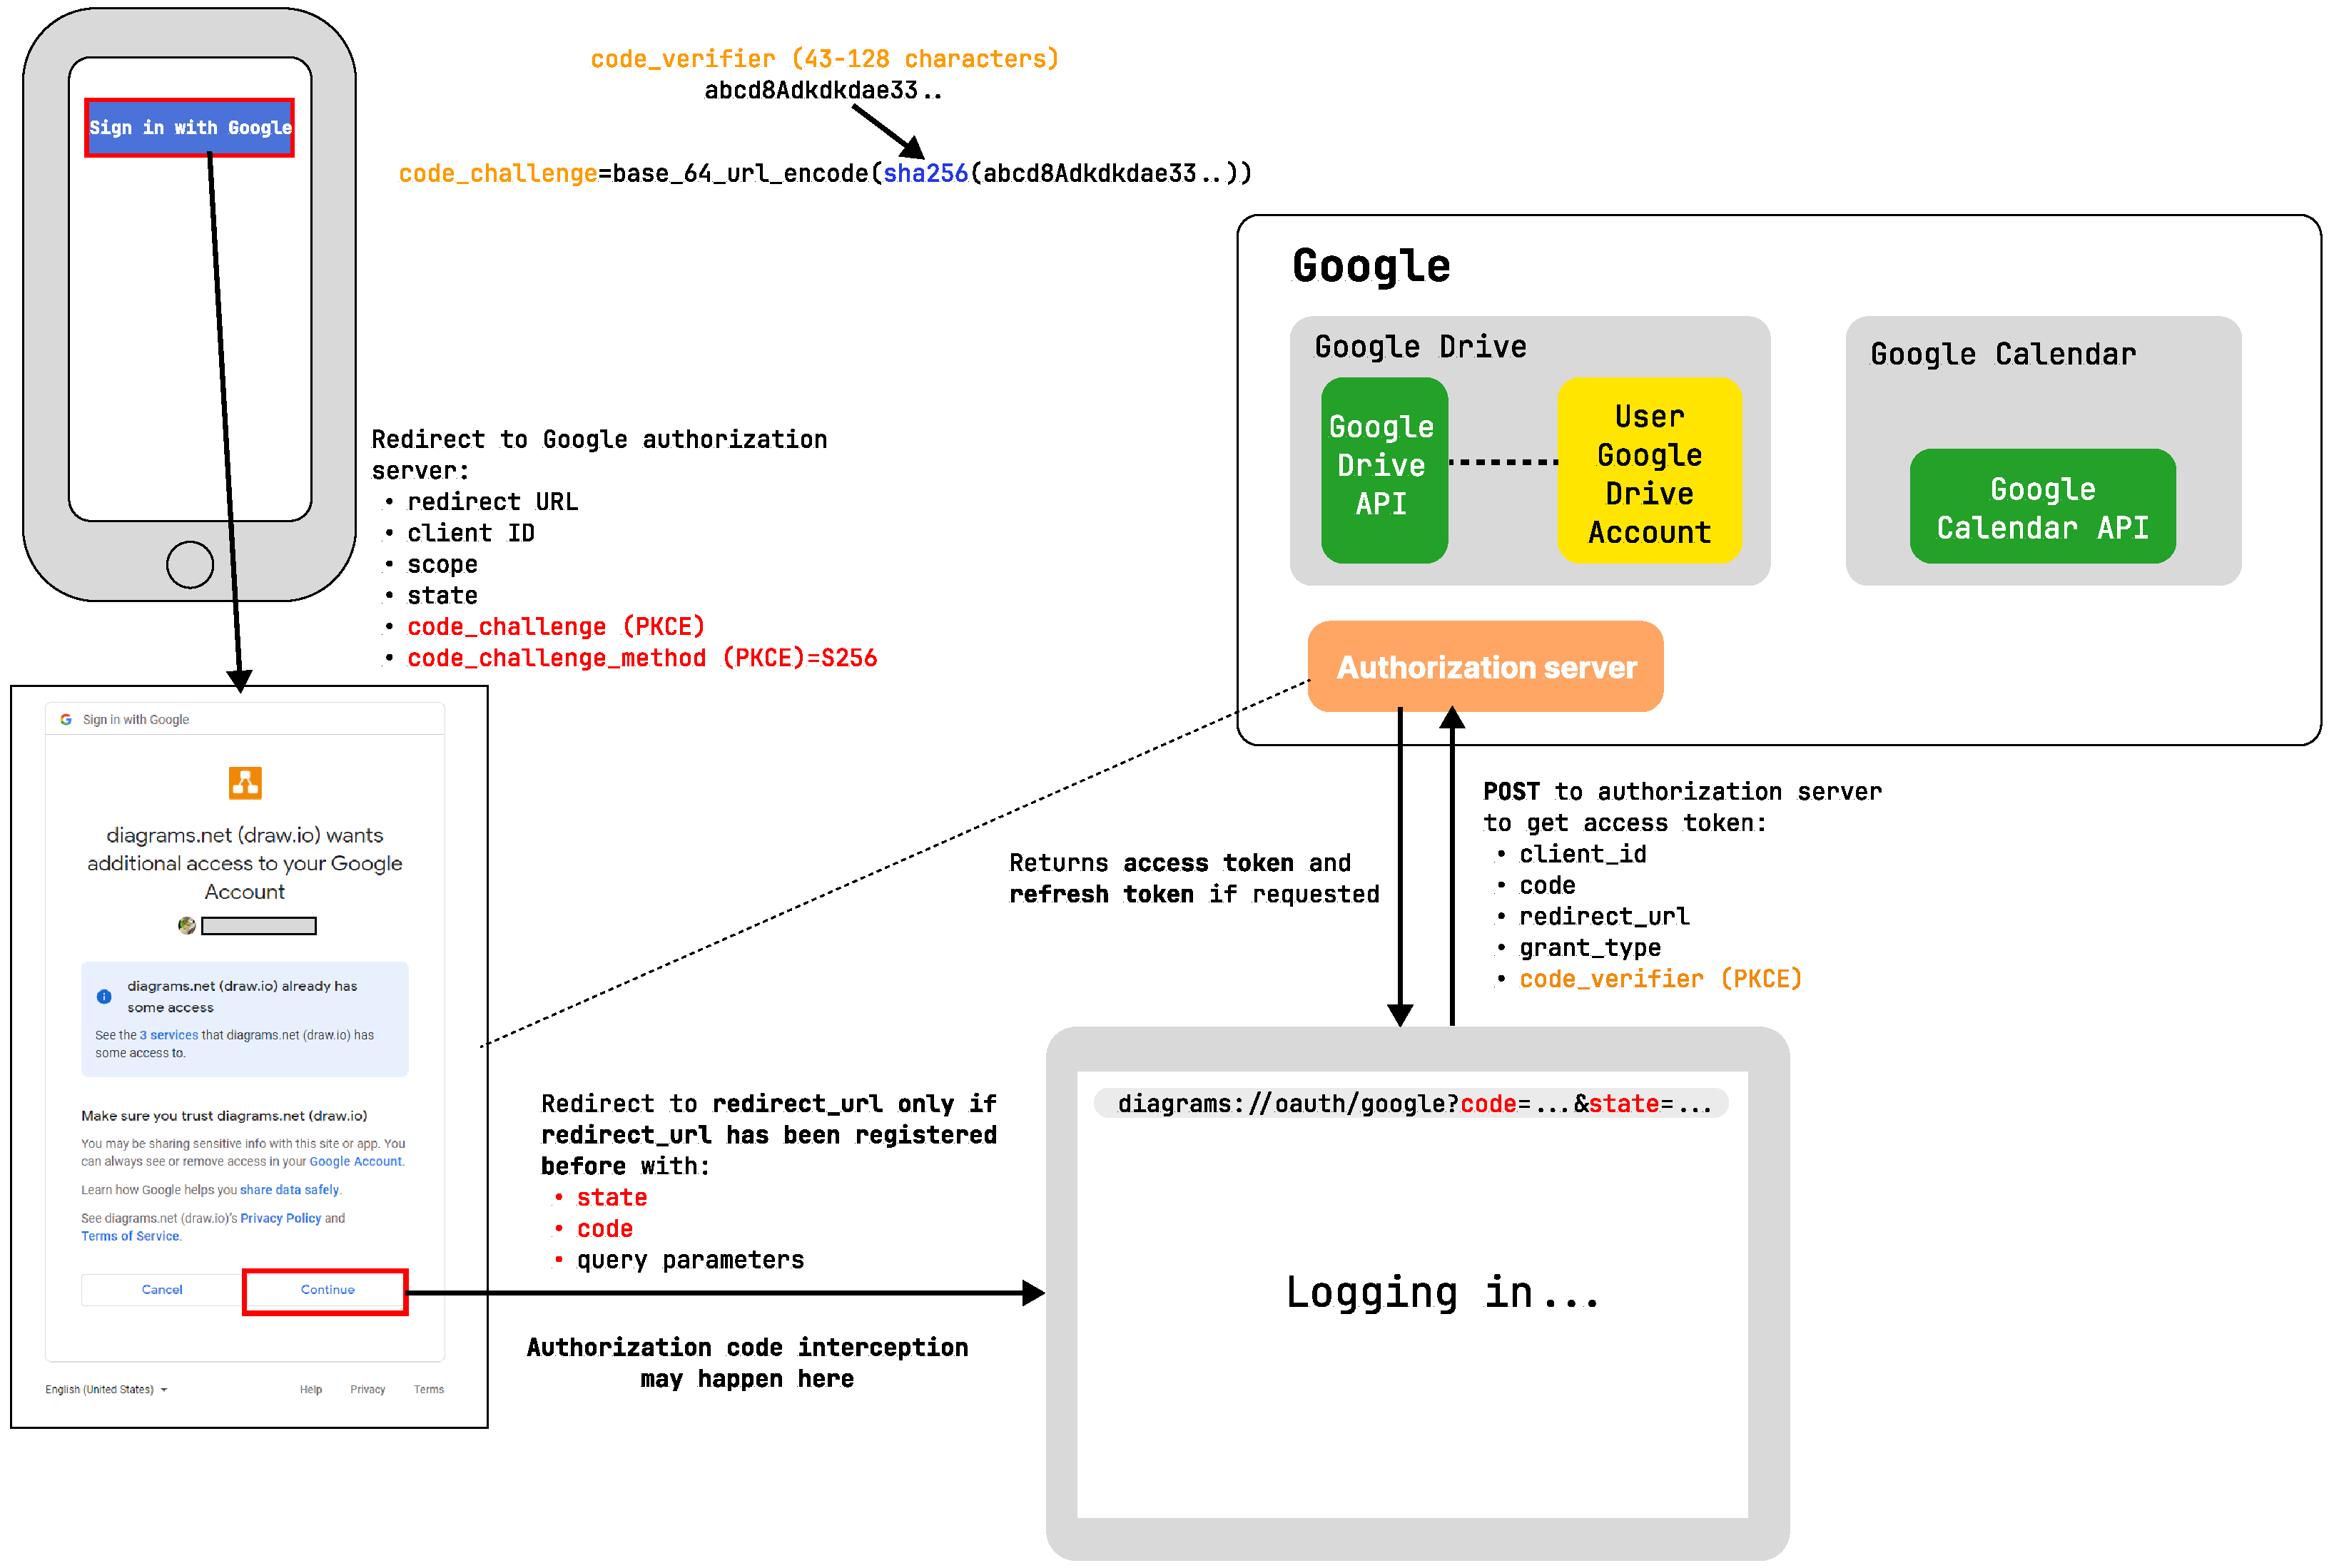
\includegraphics[width=1\textwidth]{img/OAuthPkceScheme_1570_1055}
    ~\caption{OAuth 2.0 with PKCE flow diagram.}
\end{figure}

\begin{enumerate}
    \item After clicking on the \texttt{Sign in with Google} button,
    the browser is redirected to the authorization endpoint, where the resource owner (user) enters credentials e.g., login and password.
    \item After successful authentication, the browser is redirect to \texttt{redirect\_uri} defined in OAuth provider settings.
    The \texttt{code} parameter is attached to the request parameters.
    \item Having the \texttt{code} value application exchanges it to a pair of access and refresh tokens.
    If we used PKCE with specified \texttt{code\_challenge} and \texttt{code\_challenge\_method} values exchanging code to a pair of tokens,
    we must pass the value of \texttt{code\_verifier} to the request.
\end{enumerate}
We mention here such definitions as code and state, and they mean
\begin{itemize}
    \item \textbf{Code} is an authorization code that is obtained through an authorization
    server and mediates between clients and resource owners.
    Before the authorization server redirects the resource owner back to the client,
    the authorization server verifies the authenticity of the resource owner.
    So because the resource owner only authenticates with the authorization server,
    their credentials are never sent to the client.
    \item \textbf{State} is the value used by the client to store the state between the authorization request and the callback.
    The authorization server enables this value when redirecting the user agent back to the client.
    This parameter is used to prevent CSRF attacks.
\end{itemize}

Adding the Proof of Key Code Exchange (PKCE) to the OIDC flow improves protocol security so that the code
cannot be exchanged by third-party applications by-passing the original application.
Authorization code flow with PKCE is a protocol that represents a client-generated secret that can be verified
by an authorization server.
This secret is called \texttt{code\_verifier}.
The client hashes the \texttt{code\_verifier} value and writes it to the \texttt{code\_challenge} parameter
of an HTTP request.
PKCE solves the problem of secure code exchange.
If an attacker manages to get an authorization code, then he will not be able to exchange
it for access and refresh tokens.
Therefore, we ensure that the exchange of a code for tokens is produced by the same application
that performed the authentication.
Proof of Key Code Exchange can be compared to the digital signature of an authentication process.
To exchange the \texttt{code} for a pair of access and refresh tokens, it is necessary to specify
a valid \texttt{code\_verifier}.